
\documentclass[oneside,a4paper]{book}
%\pagestyle{headings}


%=============================================================================

\usepackage{amsthm}
\usepackage{xspace}
\usepackage{float}
\usepackage{ifthen}
\usepackage{amsbsy}
\usepackage{amssymb}
\usepackage{balance}
\usepackage{booktabs}
\usepackage{graphicx}
\usepackage{rotating}
\usepackage{multirow}
\usepackage{needspace}
\usepackage{microtype}
\usepackage{bold-extra}
\usepackage{geometry}
\usepackage{varioref}
\usepackage{xcolor}
\usepackage{textcomp}
\usepackage{listings}
\usepackage[normalem]{ulem} %emphasize still italic
\usepackage{ucs}
\usepackage{booktabs}

% \usepackage[utf8]{inputenc}
% \usepackage[htt]{hyphenat}
\usepackage{times}
\usepackage{url}
\usepackage{alltt}
\usepackage{amsmath}
\usepackage{xfrac}
\usepackage{subfigure}
\usepackage{appendix}
\usepackage{stmaryrd}   % for the \shortuparrow
\usepackage[utopia]{quotchap}

\usepackage{setspace}
\usepackage[numbers, sort&compress]{natbib}
\usepackage{mdwlist}        % support for better spaced lists
% allows for temporary adjustment of side margins
\usepackage{chngpage}
\usepackage[normalem]{ulem} 

% constants

\newcounter{qcounter}

% commands
\newcommand{\n}{$\cdot$}
\newcommand{\y}{\checkmark}
\newcommand{\subscript}[1]{$_{\textrm{\footnotesize{#1}}}$}
\newcommand{\superscript}[1]{$^{\textrm{\footnotesize{#1}}}$}
\newcommand{\vertical}[1]{\raisebox{-4em}{\begin{sideways}{#1}\end{sideways}}}

\newboolean{showedits}
\setboolean{showedits}{true} % toggle to show or hide edits
\ifthenelse{\boolean{showedits}}
{
       \newcommand{\ugh}[1]{\textcolor{red}{\uwave{#1}}} % please rephrase
       \newcommand{\ins}[1]{\textcolor{blue}{\uline{#1}}} % please insert
       \newcommand{\del}[1]{\textcolor{red}{\sout{#1}}} % please delete
       \newcommand{\chg}[2]{\textcolor{red}{\sout{#1}}{\ra}\textcolor{blue}{\uline{#2}}} % please change
}{
       \newcommand{\ugh}[1]{#1} % please rephrase
       \newcommand{\ins}[1]{#1} % please insert
       \newcommand{\del}[1]{} % please delete
       \newcommand{\chg}[2]{#2}
}


% ============================================================================
% Put edit comments in a really ugly standout display

\usepackage{xcolor}
\usepackage[normalem]{ulem}
\newcommand{\ra}{$\rightarrow$}


% comments \nb{label}{color}{text}
\newboolean{showcomments}
\setboolean{showcomments}{true}
\ifthenelse{\boolean{showcomments}}
    {\newcommand{\nb}[3]{
        {\colorbox{#2}{\bfseries\sffamily\scriptsize\textcolor{white}{#1}}}
        {\textcolor{#2}{\sf\small$\blacktriangleright$\textit{#3}$\blacktriangleleft$}}}
     \newcommand{\version}{\emph{\scriptsize$-$Id$-$}}
%	 \newcommand{\ugh}[1]{\textcolor{red}{\uwave{#1}}} % please rephrase
%	 \newcommand{\ins}[1]{\textcolor{blue}{\uline{#1}}} % please insert
%	 \newcommand{\del}[1]{\textcolor{red}{\sout{#1}}} % please delete
%	 \newcommand{\chg}[2]{\textcolor{red}{\sout{#1}}{\ra}\textcolor{blue}{\uline{#2}}} % please change
	 \newcommand{\chk}[1]{\textcolor{ForestGreen}{#1}} % changed, please check
	}
    {\newcommand{\nb}[3]{}
     \newcommand{\version}{}
	\newcommand{\chk}[1]{} % changed, please check
	}

% ============================================================================
% Make quotes be italic
\renewenvironment{quote}
    {\list{}{\rightmargin\leftmargin}%
     \item\relax\begin{it}}
    {\end{it}\endlist}

\newcommand{\ttimes}{\ensuremath{\times}}

%=============================================================================

\newcommand{\needlines}[1]{\Needspace{#1\baselineskip}}

% source code
\usepackage{xcolor}
\usepackage{textcomp}
\usepackage{listings}
\definecolor{source}{gray}{0.9}
\lstset{
	language={},
	% characters
	tabsize=3,
	upquote=true,
	escapechar={!},
	keepspaces=true,
	breaklines=false,
	alsoletter={:},
	breakautoindent=true,
	columns=fullflexible,
	showstringspaces=false,
	basicstyle=\footnotesize\ttfamily,
	% background
	frame=single,
    framerule=0pt,
	backgroundcolor=\color{source},
	% numbering
	numbersep=5pt,
	numberstyle=\tiny,
	numberfirstline=true,
	% captioning
	captionpos=b,
	numberbychapter=false,
	% formatting (html)
	moredelim=[is][\textbf]{<b>}{</b>},
	moredelim=[is][\textit]{<i>}{</i>},
	moredelim=[is][\uline]{<u>}{</u>}}
\newcommand{\ct}{\lstinline[backgroundcolor=\color{white},basicstyle=\footnotesize\ttfamily]}
\newcommand{\lct}[1]{{\small\tt #1}}


%----------------------------------------------------------------------------
% references
\newcommand{\tabref}[1]{\hyperref[{tab:#1}]{Table~\ref*{tab:#1}}}
\newcommand{\figref}[1]{\hyperref[{fig:#1}]{Figure~\ref*{fig:#1}}}
\newcommand{\secref}[1]{\hyperref[{sec:#1}]{Section~\ref*{sec:#1}}}
\newcommand{\lstref}[1]{\hyperref[{lst:#1}]{Listing~\ref*{lst:#1}}}
\newcommand{\charef}[1]{\hyperref[{cha:#1}]{Chapter~\ref*{cha:#1}}}
%----------------------------------------------------------------------------

% abbreviations
\tracingcolors 4
\setcounter{tocdepth}{3}
\setcounter{secnumdepth}{3}
\newcommand{\ie}{\emph{i.e.,}\xspace}
\newcommand{\eg}{\emph{e.g.,}\xspace}
\newcommand{\etc}{\emph{etc.}\xspace}
\newcommand{\etal}{\emph{et al.}\xspace}


\newcommand{\newevenside}{
	\ifthenelse{\isodd{\thepage}}{\newpage}{
	\newpage
        \phantom{placeholder} % doesn't appear on page
	\thispagestyle{empty} % if want no header/footer
	\newpage
	}
}

\def\stretchfactor{1}
\newcommand{\mychapter}[1]{\setstretch{1}
    \chapter{#1}\setstretch{\stretchfactor}}

%----------------------------------------------------------------------------
\newcommand{\lessSpace}{\vspace{-1em}}
\DeclareGraphicsExtensions{.pdf,.png}
\graphicspath{{images/}}
\newcommand{\fig}[4]{
	\begin{figure}[#1]
		\centering
		\includegraphics[width=#2\textwidth]{#3}
		\lessSpace
		\caption{\label{fig:#3}#4}
	\end{figure}}

% ===========================================================================


\newcommand{\thesistitle}{Automating high-quality translations for Mobile Apps}
\newcommand{\thesisauthor}{Wanzenried \& Stefan}
\newcommand{\thesisleiter}{Prof. Dr. Philippe Cudr\'{e}-Mauroux}
\newcommand{\thesisasst}{Roman Prokofyev}
\newcommand{\thesissubtitle}{}
\newcommand{\thesisdate}{May 2016}



% ===========================================================================

\usepackage[ colorlinks=true, urlcolor=black, linkcolor=black,
			citecolor=black, bookmarksnumbered=true, bookmarks=true,
			plainpages=false,
			pdftitle={\thesistitle}, pdfauthor={\thesisauthor},
			pdfsubject={\thesissubtitle}, pdfpagelabels]{hyperref}

\newcommand{\hrref}[2]{\hyperref}
% ===========================================================================
% ===========================================================================


% D O C U M E N T
% % % % % % % % % % % % % % % % % % % % % % % % % % % % % % % % % %
\begin{document}

% T I T L E
% % % % % % % % % % % % % % % % % % % % % % % % % % % % % % % % % %
\begin{titlepage}  
  \begin{center}  
  
  \begin{figure}[t]  
  \vspace*{-2cm}        % to move header logo at the top 
  \center{
\includegraphics[scale=0.2]{logos/MSc_quer.png}}
  \vspace{0.4in}     
  \end{figure}

    \thispagestyle{empty}
    
    {\bfseries\Huge \thesistitle \par
    \Large \vspace{0.1in} \thesissubtitle \par}

    \vspace{0.3in} 
    \LARGE{\textbf{Master Thesis} \\}
    \vspace{0.4in}

    {\Large \thesisauthor \par from \par Bern BE, Switzerland}
    
    \vspace{0.3in}
%    {\Large Home University \par}
    {\Large Philosophisch-naturwissenschaftliche Fakult\"{a}t \\
            der Universit\"{a}t Bern \par}
    \vfill
    {\Large \thesisdate \par}
    \vspace{0.3in}
    %Leiter der Arbeit: \par
%   {\Large \thesisleiter, Research Group, Institute, University, Supervisor}\par
   {\Large \thesisleiter, eXascale Infolab, University of Fribourg, Switzerland, Supervisor}\par
   {\Large \thesisasst, eXascale Infolab, University of Fribourg, Switzerland, Assistant}
  

  \vspace{0.9in}
 
  % === Logos ==============================================     
  \begin{figure}[htp]
    \centering
    
\includegraphics[scale=0.30]{logos/UNI_Bern.png}\hfill
    
\includegraphics[scale=0.30]{logos/UNI_Neuenburg.png}\hfill
    
\includegraphics[scale=0.80]{logos/UNI_Fribourg.png}
  \end{figure}
  % === // Logos ===========================================    


  \end{center}

\end{titlepage}


% A B S T R A C T
% % % % % % % % % % % % % % % % % % % % % % % % % % % % % % % % % %
\chapter*{\centering Abstract}
\begin{quotation}
\noindent 
Every day, hundreds of mobile applications are added to stores such as Google Play or AppStore. Many of them are intended to be used internationally, and thus require translation of the interface. At the same time, many more mobile apps already available for download in these stores. Leveraging the translation bases of existing applications, we could immediately provide high-quality translations for new apps without need to go though a human-translation process. 

This project aims to extract and parse translations of existing applications to see if they can be used to translate new ones. A prototype application allows to translate existing apps from a given source to a target language. Translations are generated with different algorithms in statistical machine translation.
\end{quotation}
\clearpage


% C O N T E N T S 
% % % % % % % % % % % % % % % % % % % % % % % % % % % % % % % % % % % % % % % %
\tableofcontents

%%%%%%%%%%%%%%%%%%%%%%%%%%%%%%%%%%
%%%% NEW CHAPTER %%%%%%%%%%%%%%%%%%%%%
%%%%%%%%%%%%%%%%%%%%%%%%%%%%%%%%%%
\chapter{Introduction}
\label{cha:introduction}

Android and iPhone smartphones are available in countries all over the world. If an app is intended to be used internationally, translating it into multiple languages can be important to attract more users. If people understand the app better, they may leave higher ratings. However, translating an app requires additional effort. From the developers perspective, all strings must be isolated in order to replace them with different values for each supported language. Furthermore, translating all text itself is a difficult task which usually requires the work of a professional translator. // TODO 

This thesis focus on automatic translations of Android apps from English to French and German. The main idea is to collect a lot of existing apps from the Google Playstore\footnote{\url{https://play.google.com/store}} and extract their translations. Are we able to provide high quality translations with the help of statistical machine translation (SMT) systems? In order to produce good translations, SMT system must consist of a big vocabulary. It is therefore assumed that apps belonging to the same categories (e.g. finance, audio, sport etc.) share similar translations. SMT is the dominant approach in automating translations and used by services like Google Translate\footnote{\url{https://translate.google.com}} and Bing Translator\footnote{\url{https://www.bing.com/translator}} (Microsoft). In this thesis, we use different SMT algorithms to generate translations. A prototype web application is built which serves as a playground to translate strings and compare the results. Finally, the results of different translation systems are compared and the translation quality is evaluated with the BLEU metric.

\chapter{Problem Analysis}
\label{cha:problem_analysis}

// TODO

\section{Android apps and internationalization}

Android uses a key-value based approach to store translations and other resources in XML files\footnote{\url{http://developer.android.com/guide/topics/resources/localization.html}}. For each supported language, one XML file exists, containing the translated values to the given keys. In the source code, a string is no longer hardcoded but referenced by a translation key.

// TODO

\section{Challenges}

- Quality of existing translations?
- Where and how to obtain large amount of apps
- Hardware for SMT systems. Training may need a lot of time
- How many data is needed to produce good results?
- How can we measure good translations?


\chapter{Data Analysis}

\section{Apps}

A total of 698 free Android apps were collected from various categories\footnote{Click on Categories to see a list of available categories at:  \url{https://play.google.com/store/apps?hl=en}}, ensuring a good mix of different translations. Most of them were chosen randomly beside the top apps, mostly from Google, that ensure good translation quality of different languages. Figure \ref{fig:data_analysis_top_apps_en} shows the top ten apps according to the number of available english translations. Note that the counts indicate the number of effective translations after eliminating uninteresting data during pre-processing the corpus (see. chapter XY). Most of the apps have similar counts for all the three languages. Surprisingly, some apps provide more translations for german and french than english. Different counts can happen because of:

\begin{enumerate}
\item Not all strings were translated to all languages. Some english words don't need to be translated, e.g. E-Mail.
\item Some translations were abandoned during pre-processing.
\item The XML files containing the translations are out of sync.
\end{enumerate}

34 apps did not isolate their strings in XML files (we assume that they are hardcoded in the programming code). This leaves a effective number of 664 apps where we could extract translations. However, 241 apps were not multilingual and therefore not useful for building translation systems. Unfortunately, apps are not marked as multi-language in the app store, so we only know if there are translations available after downloading and extracting the data.

\begin{figure}[H]
    \centering
    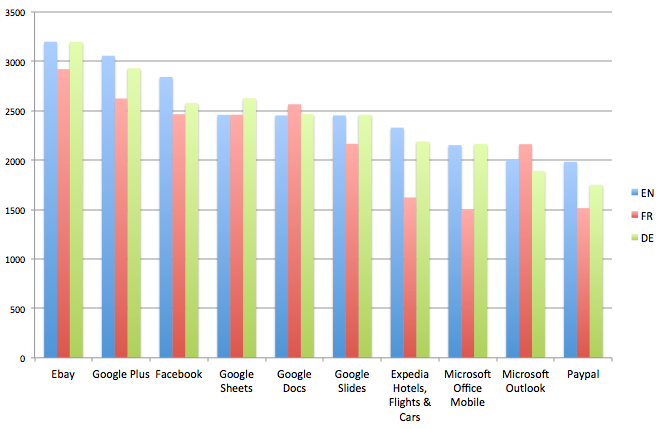
\includegraphics[width=0.75\textwidth]{images/data_analysis_top_apps_en.png}
    \caption{Top apps by the number of english translations}
    \label{fig:data_analysis_top_apps_en}
\end{figure}


\section{Languages}

We collected a total of 423 multilingual apps, offering its content at least for two languages. Figure \ref{fig:data_analysis_n_langs} shows the number of apps for the ten most used languages. French and German, where we focus on this thesis, are both in the top 4. The top apps are translated in many languages. In total, 117 different languages were used.

\begin{figure}[H]
    \centering
    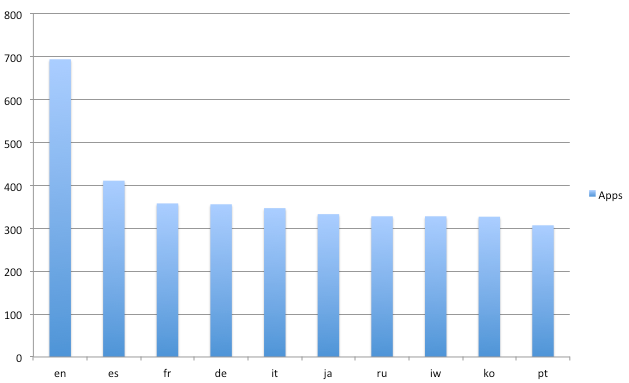
\includegraphics[width=0.75\textwidth]{images/data_analysis_languages_count.png}
    \caption{Number of apps available in the top ten languages.}
    \label{fig:data_analysis_n_langs}
\end{figure}



\section{Top Terms}




\begin{table}[H]
\centering
\resizebox{\textwidth}{!}{%
\begin{tabular}{@{}llllllll@{}}
\toprule
EN & Count &  & FR & Count &  & DE & Count \\ \midrule
Cancel & 1894 &  & Annuler & 1067 &  & Abbrechen & 886 \\
Done & 1230 &  & Supprimer & 745 &  & Google Play-Dienste aktivieren & 730 \\
Settings & 1102 &  & Connexion & 745 &  & Google Play-Dienste installieren & 728 \\
Search & 884 &  & Mettre à jour & 486 &  & Anmelden & 664 \\
Delete & 704 &  & Rechercher & 485 &  & Löschen & 664 \\
Enable Google Play services & 692 &  & Paramètres & 450 &  & Aktualisieren & 652 \\
Get Google Play services & 690 &  & Mettre à jour les services Google Play & 370 &  & Einstellungen & 569 \\
Log Out & 556 &  & Activer services google Play & 368 &  & Fertig & 548 \\
Update & 545 &  & Activer les services Google Play & 366 &  & Weiter & 484 \\
Share & 541 &  & Installer les services Google Play & 366 &  & Schliessen & 428 \\ \bottomrule
\end{tabular}
}
\caption{Top ten terms for english, french and german}
\label{table:data_analysis_top_terms}
\end{table}

\chapter{Data extraction, preparation and storage}


\section{Extract translations}

An android app has the form of a single binary file (suffix .apk). The XML files containing the translations are packed inside the .apk file. We used a software called ``Apktool''\footnote{\url{http://ibotpeaches.github.io/Apktool/}} to reverse engineer existing apps and extract the needed XML files.

\section{Pre-process translations}

This task involves two parts. First of all, the translations are sanitized from unwanted information such as HTML tags. Some strings are omitted at this stage because they do not provide any meaningful value to the translation process, for example URLs or placeholders combined with plain numbers. Secondly, the sanitized strings are prepared to be read by an SMT system.

\subsection{Sanitizing}

The following rules are used to get rid of unwanted translations or parts of it:

\begin{itemize}
\item Trim the string from newlines (\texttt{\textbackslash n}), tabs (\textbackslash t) or carriage return (\textbackslash r)
\item Strip any HTML tags
\item Omit strings that are URLs (starting with http or www)
\item Remove strings placeholders like \texttt{\%s} or \texttt{\%1\$s}
\item Ignore words with less than 3 characters
\item Finally, the resulting string is trimmed again from spaces and must contain at least one alphanumerical character
\end{itemize}


\subsection{Tokenization and Truecasing}

Tokenization is required to separate words from punctuation. Each token is separated by a space character: ``\texttt{Hi, my name is John.}'' becomes ``\texttt{Hi , my name is John .}''

After tokenizsation, we applied Truecasing to our text corpus.\footnote{\url{https://en.wikipedia.org/wiki/Truecasing}} In contrast to lowercasing, truecasing determines the proper capitalization of words. This is done by analyzing all data first and then apply the most likely capitalization. It is especially useful for words starting a sentence, that are written uppercase in many languages. For example the word ``\texttt{This}'' starting a sentence will then be recognized as ``\texttt{this}'' by an SMT system.


\section{Data storage}

All translations are stored in text files. Additionally, each translation is stored in a document with Apache Solr\footnote{\url{http://lucene.apache.org/solr/}}. Solr is an open source text search platform built on top of Apache Lucene\footnote{\url{https://lucene.apache.org/core/}}.

\subsection{Corpus}

After pre-processing the translations, they are written to text files, one sentence per line. The corpus is split into parallel and monolingual data. Parallel data of two language pairs contains two text files, one for each language. All sentences must be aligned so that line x of the target language corresponds to line x of the source language. A SMT system uses this parallel data to train the translation model.
In addition, data of any language is stored monolingual. All sentences are written into one single text file. This is for example used to build language models. // TODO 

\subsection{Apache Solr}

Solr allows to store the translations with additional meta data, such as the translation key and a unique app ID. Due to its way of indexing text data, Solr is very fast when querying translations. Furthermore, built in tools allow us to get nice statistics about our translations, for example the top terms grouped by language.
// TODO

\subsubsection{Setup and schema}

Solr offers so called "Cores" where each core manages a separate index, schema and configuration\footnote{\url{https://cwiki.apache.org/confluence/display/solr/Solr+Cores+and+solr.xml}}. In our setup we created one core per language holding all the translations. The schema is identical for each core and consist of the following fields:

\subsubsection{Queries}



\chapter{Statistical machine translation SMT}

\section{Phrase-based}

\subsection{Moses}

\section{Deep learning}

\subsection{Tensorflow}

\chapter{Prototype web application}

\subsection{Architecture}

\subsection{Frontend}

\chapter{Evaluation}

\section{Comparing results}

\section{BLEU score}


%\chapter {Related Work}
%In which we learn what have other done to address similar problems. For example, the work of Star \cite{Star89}
%
%\chapter{The Problem}
%In which we understand what the problem is in detail.
%
%\chapter {The Solution}
%In which you describe your solution.
%
%\chapter {The Validation}
%In which you show how well the solution works.
%
%\chapter {Conclusion and Future Work}
%In which we step back, have a critical look at the entire work, then conclude, and learn what lies beyond this thesis.



%END Doc
%-------------------------------------------------------

\bibliography{thesis}
\bibliographystyle{plain}

\end{document}
